\documentclass[12pt]{article}

\usepackage{graphicx,url}

\usepackage[brazilian]{babel}   
\usepackage[utf8]{inputenc}
\usepackage[T1]{fontenc}
\usepackage{hyperref}
\usepackage{float}
\usepackage{booktabs}
\usepackage{abntex2cite}
\usepackage{amsmath}
\usepackage{textcomp}



%opening
\title{Otimização não linear}
\author{Felipe Duarte dos Reis}

\begin{document}

\maketitle

\begin{abstract}
Apresentação dos resultados para o método de Newton, Newton com correção do posto, e quasi-Newton.
\end{abstract}

\section{Introdução}
Este relatório apresenta o resultado da execução dos três métodos de otimização (Newton modificado, Newton com correção do posto e Quasi-Newton) para as 
doze funções entregues em sala. Todas as execuções começaram no ponto inicial $ \begin{bmatrix} 3 & 5 \end{bmatrix}^T $. A precisão do cálculo foi de $1e-3$ 
e as condições de parada adotadas foram a norma do vetor gradiente ser menor que $1e-3$ ou o algoritmo atingir o número máximo de iterações igual a 100. 
Para calcular os vetores gradientes foi utilizado um $\Delta = 1e-6$.

\section{Função 1}
A regra que define a função é:
\begin{equation}
\label{eq:f1}
f(x, y) = 
	   \begin{bmatrix}
            x - 2 & y - 1
           \end{bmatrix}            
           \begin{bmatrix}
	   2 	& 0,2 \\
	   0,3	& 4 
           \end{bmatrix} 
           \begin{bmatrix}
	   x - 2 \\
	   y - 1
           \end{bmatrix}
\end{equation}

Podemos ver na \autoref{fig:f1} as curvas de nível para \autoref{eq:f1}. O símbolo \textit{\textopenbullet} marca o ponto de início,
e o símbolo \textit{\texttimes} marca o ótimo encontrado pelos três algoritmos. 

\begin{figure}[H]
  \centering
  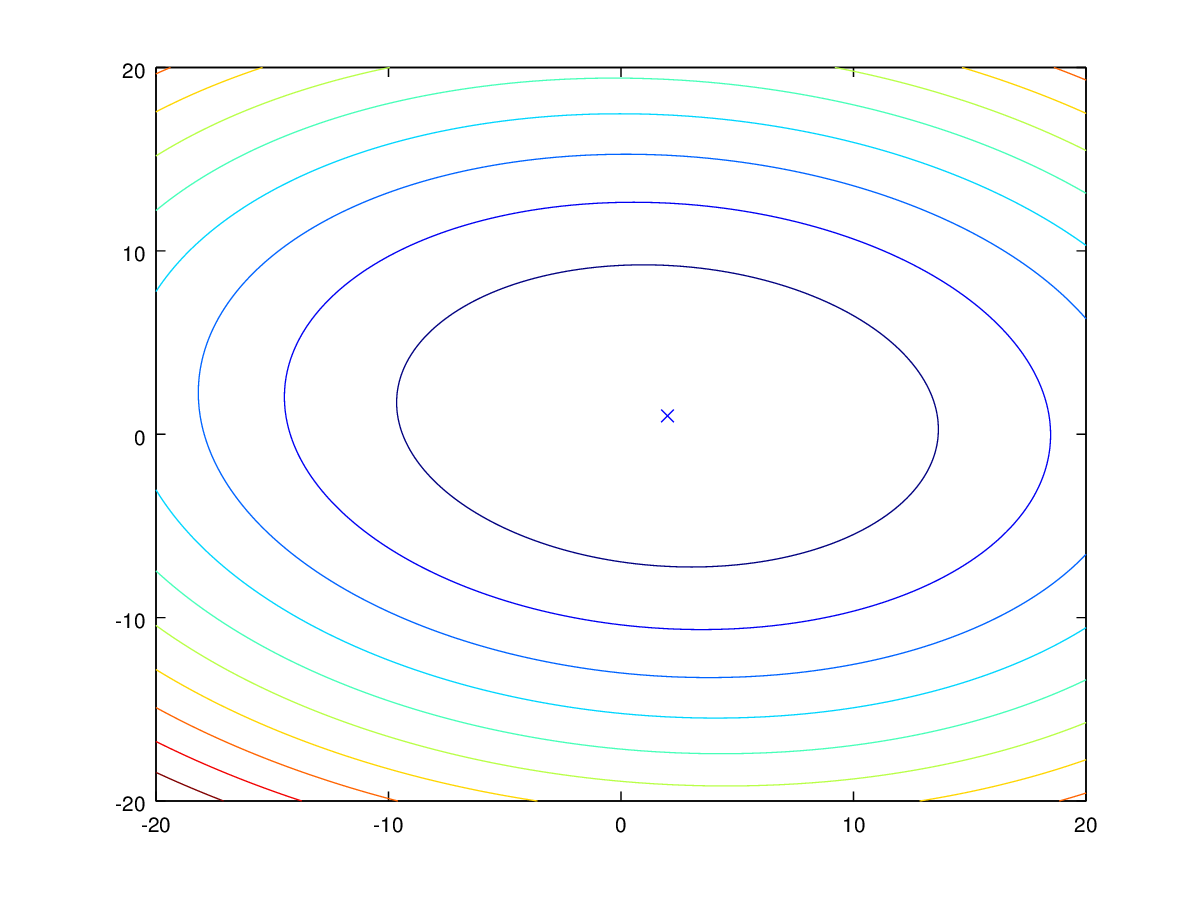
\includegraphics[width=250px]{../matlab/images/f1_contour}
  \caption{Curvas de nível para a função \autoref{eq:f1}}
  \label{fig:f1}
\end{figure}

A \autoref{tab:f1} mostra os resultados encontrados para os três algoritmos testados bem como o número de iterações gasto por cada um deles.

\begin{table}[H]
\centering
\begin{tabular}{*3c}
\toprule
Método			&	x*		&	Iterações\\
\midrule
Newton modificado	&	(2.0, 1.0)	&	3\\
Newton corrigido	&	(2.0, 1.0)	&	3\\
Quasi-newton		&	(2.0, 1.0)	&	3\\
\bottomrule
\end{tabular}
\caption{\small{Resultados para a função \autoref{eq:f1} }}
\label{tab:f1}
\end{table}

Todos os três métodos chegaram no ótimo com poucas iterações já que a função é diferenciável e monotônica.


\section{Função 2}
A regra que define a função é:
\begin{equation}
\label{eq:f2}
f(x, y) = 
	   \begin{bmatrix}
            x - 1 & y + 1
           \end{bmatrix}            
           \begin{bmatrix}
	   1 	& 0 \\
	   0	& 100 
           \end{bmatrix} 
           \begin{bmatrix}
	   x - 1 \\
	   y + 1
           \end{bmatrix}
\end{equation}

Podemos ver na \autoref{fig:f2} as curvas de nível para \autoref{eq:f2}. O símbolo \textit{\textopenbullet} marca o ponto de início,
e o símbolo \textit{\texttimes} marca o ótimo encontrado pelos três algoritmos.

\begin{figure}[H]
  \centering
  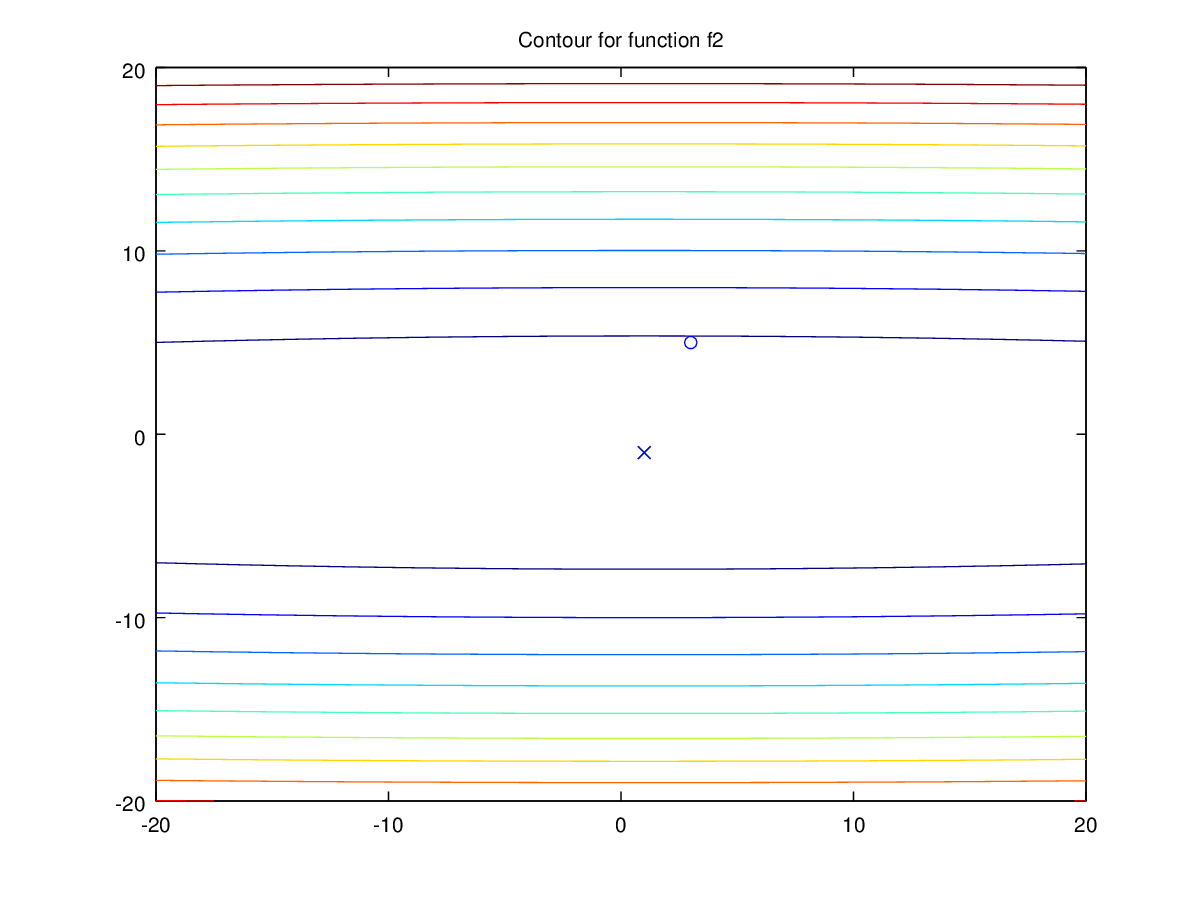
\includegraphics[width=250px]{../matlab/images/f2_contour}
  \caption{Curvas de nível para a função \autoref{eq:f2}}
  \label{fig:f2}
\end{figure}

A \autoref{tab:f2} mostra os resultados encontrados para os três algoritmos testados bem como o número de iterações gasto por cada um deles. 

\begin{table}[H]
\centering
\begin{tabular}{*3c}
\toprule
Método			&	x*		&	Iterações\\
\midrule
Newton modificado	&	(1.0, -1.0)	&	4\\
Newton corrigido	&	(1.0, -1.0)	&	4\\
Quasi-newton		&	(1.0, -1.0)	&	4\\
\bottomrule
\end{tabular}
\caption{\small{Resultados para a função \autoref{eq:f2} }}
\label{tab:f2}
\end{table}

Todos os três métodos chegaram no ótimo com poucas iterações já que a função é diferenciável e monotônica.


\section{Função 3}
A regra que define a função é:
\begin{equation}
\label{eq:f3}
f(x, y) = 
	   \begin{bmatrix}
            x + 1 & y + 2
           \end{bmatrix}            
           \begin{bmatrix}
	   1 	& 0 \\
	   0	& 0
           \end{bmatrix} 
           \begin{bmatrix}
	   x + 1 \\
	   y + 2
           \end{bmatrix}
\end{equation}

Podemos ver na \autoref{fig:f3} as curvas de nível para \autoref{eq:f3}. O símbolo \textit{\textopenbullet} marca o ponto de início,
e o símbolo \textit{\texttimes} marca o ótimo encontrado pelos três algoritmos.

\begin{figure}[H]
  \centering
  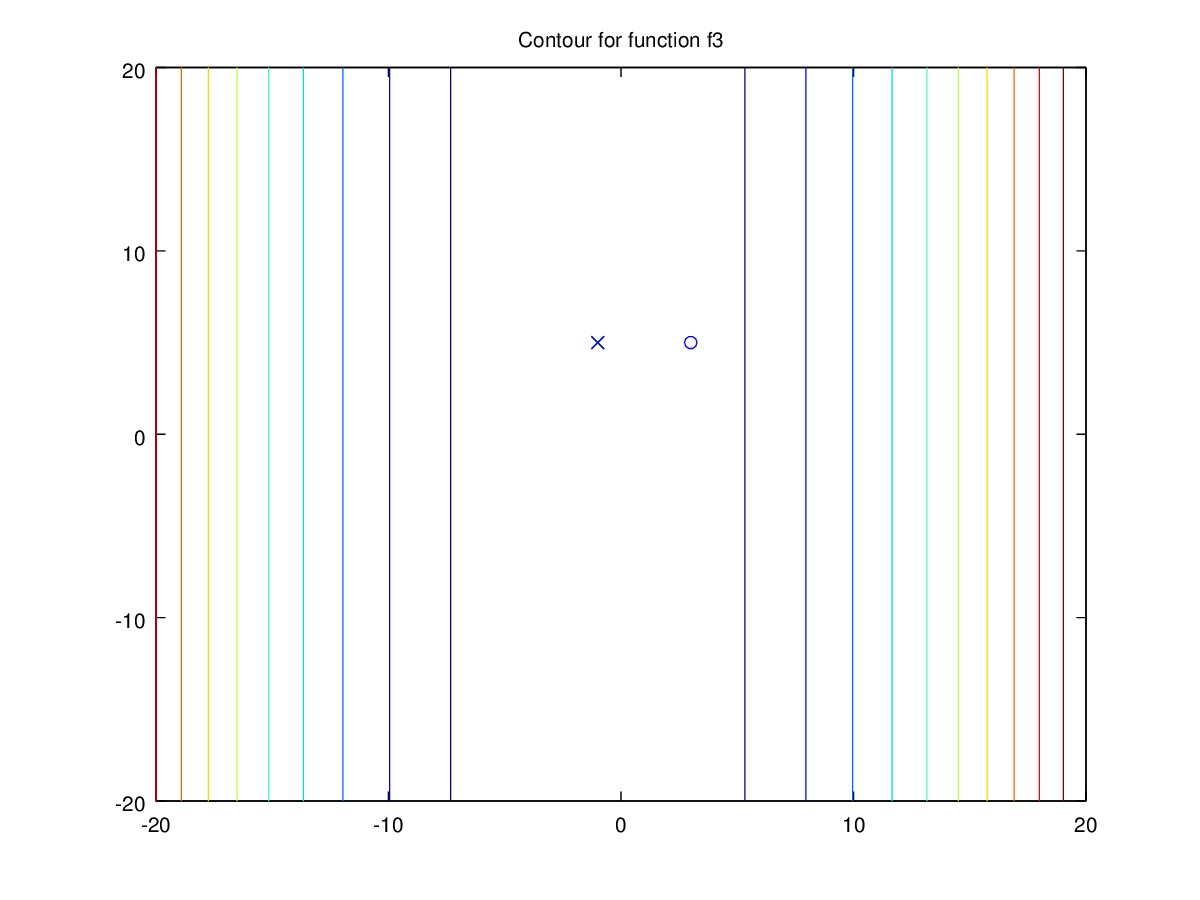
\includegraphics[width=250px]{../matlab/images/f3_contour}
  \caption{Curvas de nível para a função \autoref{eq:f3}}
  \label{fig:f3}
\end{figure}

A \autoref{tab:f3} mostra os resultados encontrados para os três algoritmos testados bem como o número de iterações gasto por cada um deles.

\begin{table}[H]
\centering
\begin{tabular}{*3c}
\toprule
Método			&	x*		&	Iterações\\
\midrule
Newton modificado	&	(-1.0, 5.0)	&	3\\
Newton corrigido	&	(-0.9999, 5.0)	&	1\\
Quasi-newton		&	(-0.9999, 5.0)	&	1\\
\bottomrule
\end{tabular}
\caption{\small{Resultados para a função \autoref{eq:f3} }}
\label{tab:f3}
\end{table}

Todos os três métodos chegaram no ótimo com poucas iterações já que a função é diferenciável e monotônica. Nesta função o método de newton não deveria convergir já que 
não é possível achar a inversa da matriz hessiana para essa função. Entretanto o método foi implementado com a função \textit{pinv()} em detrimento de \textit{inv()},
o que garante uma matriz numericamente comportada para a inversa da hessiana.

\section{Função 4}
A regra que define a função é:
\begin{equation}
\label{eq:f4}
f(x, y) = 1 - \exp(-\frac{(x+4)^2}{9} - \frac{(y-2)^2}{4})
\end{equation}

Podemos ver na \autoref{fig:f4} as curvas de nível para \autoref{eq:f4}. O símbolo \textit{\textopenbullet} marca o ponto de início,
e o símbolo \textit{\texttimes} marca o ótimo encontrado pelos três algoritmos.

\begin{figure}[H]
  \centering
  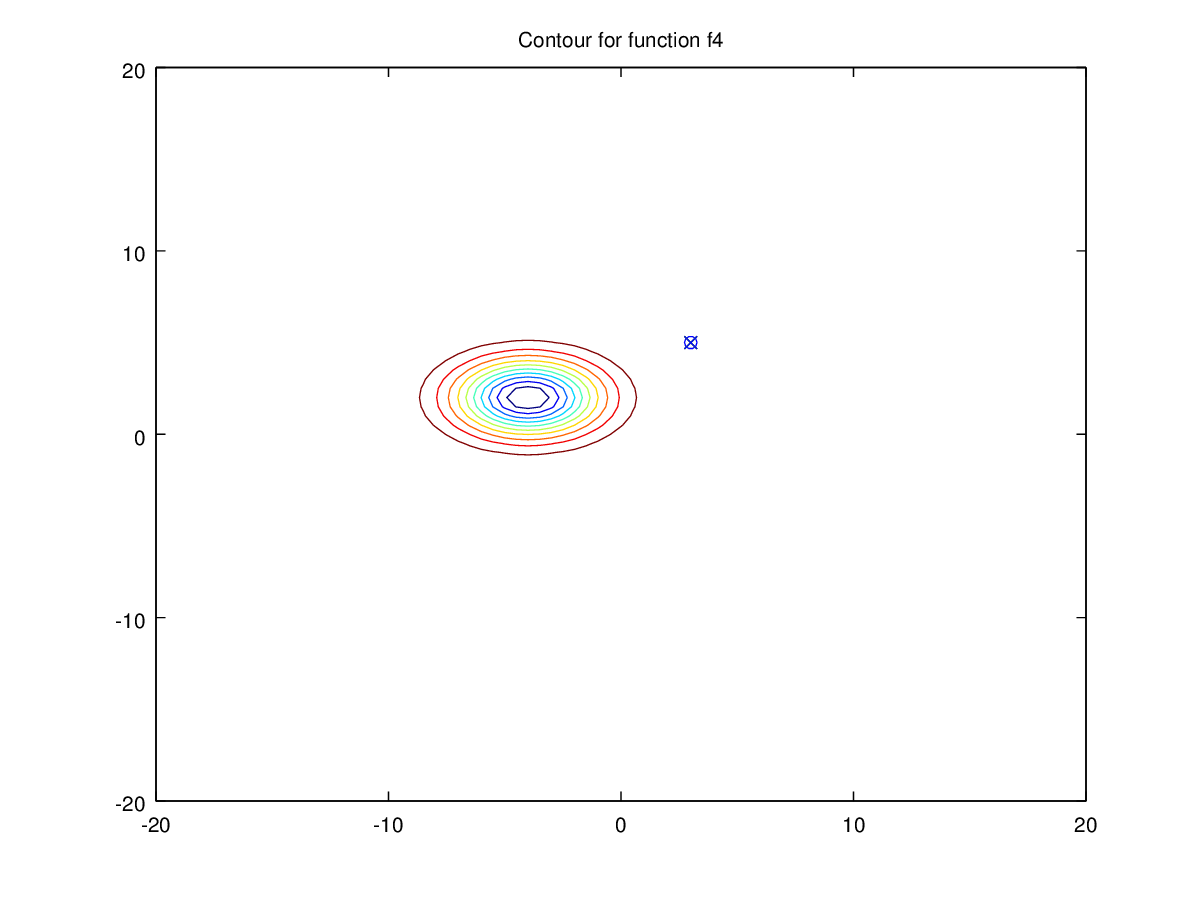
\includegraphics[width=250px]{../matlab/images/f4_contour}
  \caption{Curvas de nível para a função \autoref{eq:f4}}
  \label{fig:f4}
\end{figure}

A \autoref{tab:f4} mostra os resultados encontrados para os três algoritmos testados bem como o número de iterações gasto por cada um deles.

\begin{table}[H]
\centering
\begin{tabular}{*3c}
\toprule
Método			&	x*		&	Iterações\\
\midrule
Newton modificado	&	(3.0001, 5.0001)	&	1\\
Newton corrigido	&	(3.0000, 5.0000)	&	0\\
Quasi-newton		&	(3.0000, 5.0000)	&	0\\
\bottomrule
\end{tabular}
\caption{\small{Resultados para a função \autoref{eq:f4} }}
\label{tab:f4}
\end{table}

Apesar da função ser bem comportada, o ponto em que os métodos iniciaram não foi favorável para chegar ao mínimo global. Seria necessário
começar mais próximo da bacia de atração de forma que o algoritmo conseguisse descer até o mínimo global.

\section{Função 5}
A regra que define a função é:
\begin{equation}
\label{eq:f5}
f(x, y) = x\exp(-x^2 -y^2)
\end{equation}

Podemos ver na \autoref{fig:f5} as curvas de nível para \autoref{eq:f5}. O símbolo \textit{\textopenbullet} marca o ponto de início,
e o símbolo \textit{\texttimes} marca o ótimo encontrado pelos três algoritmos.

\begin{figure}[H]
  \centering
  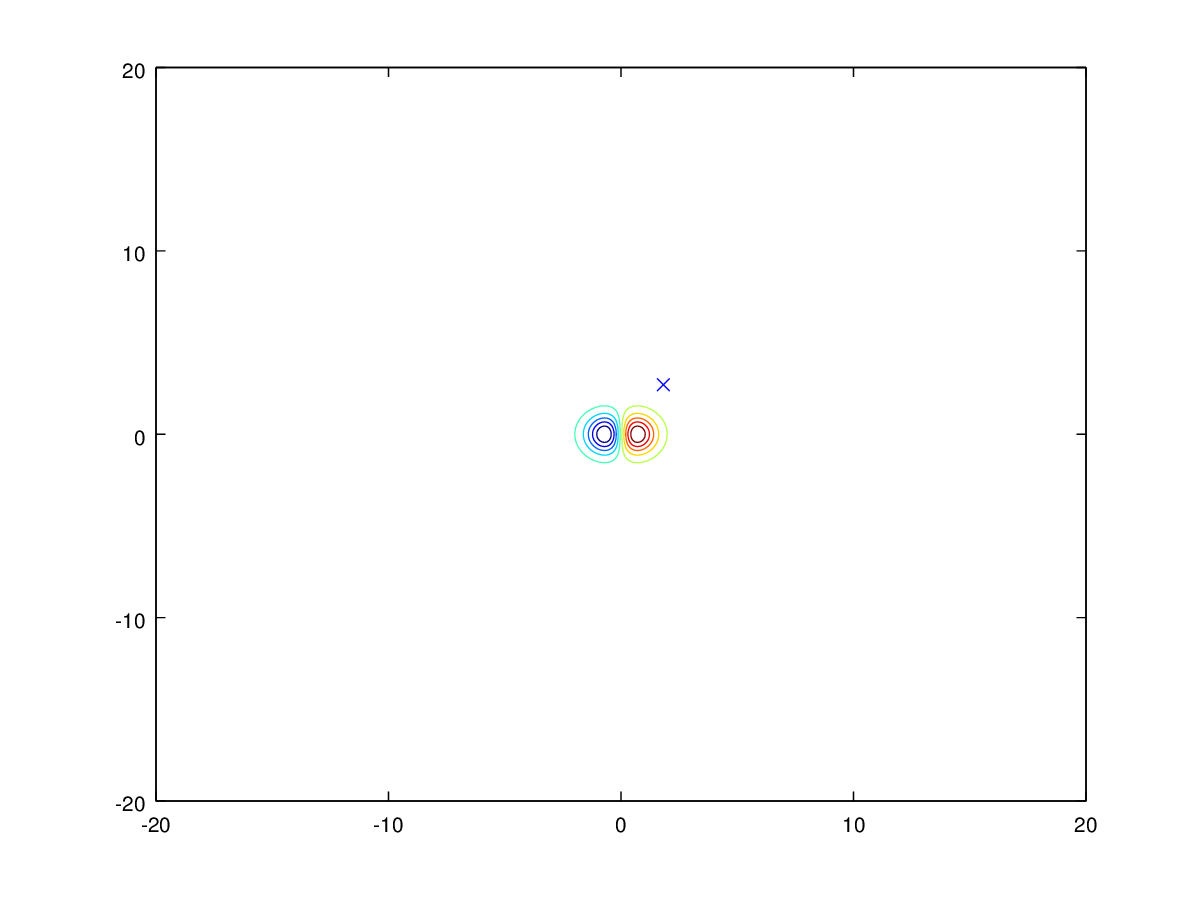
\includegraphics[width=250px]{../matlab/images/f5_contour}
  \caption{Curvas de nível para a função \autoref{eq:f5}}
  \label{fig:f5}
\end{figure}

A \autoref{tab:f5} mostra os resultados encontrados para os três algoritmos testados bem como o número de iterações gasto por cada um deles.

\begin{table}[H]
\centering
\begin{tabular}{*3c}
\toprule
Método			&	x*		&	Iterações\\
\midrule
Newton modificado	&	(3.0417, 5.0779)	&	1\\
Newton corrigido	&	(3.0000, 5.0000)	&	0\\
Quasi-newton		&	(3.0000, 5.0000)	&	0\\
\bottomrule
\end{tabular}
\caption{\small{Resultados para a função \autoref{eq:f5} }}
\label{tab:f5}
\end{table}

O mesmo que aconteceu na última função, acontece nessa. O mínimo local está muito longe do ponto de início da busca, o que faz com que
o algoritmo não consegue caminhar até a solução.

\section{Função 6}
A regra que define a função é:
\begin{equation}
\label{eq:f6}
f(x, y) = max(|x|, |y|)
\end{equation}

Podemos ver na \autoref{fig:f6} as curvas de nível para \autoref{eq:f6}. O símbolo \textit{\textopenbullet} marca o ponto de início,
e o símbolo \textit{\texttimes} marca o ótimo encontrado pelos três algoritmos.

\begin{figure}[H]
  \centering
  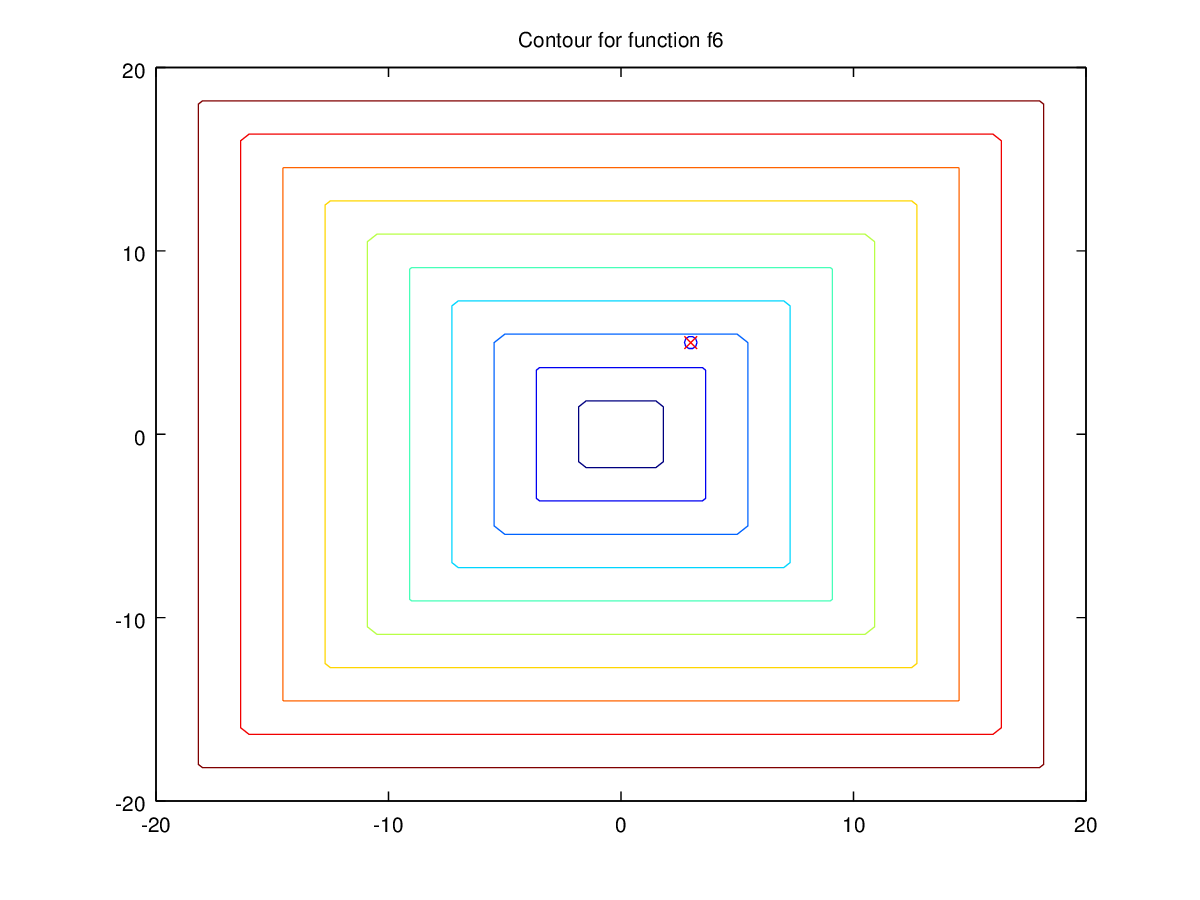
\includegraphics[width=250px]{../matlab/images/f6_contour}
  \caption{Curvas de nível para a função \autoref{eq:f6}}
  \label{fig:f6}
\end{figure}

A \autoref{tab:f6} mostra os resultados encontrados para os três algoritmos testados bem como o número de iterações gasto por cada um deles.

\begin{table}[H]
\centering
\begin{tabular}{*3c}
\toprule
Método			&	x*		&	Iterações\\
\midrule
Newton modificado	&	(3.0000, 5.0000)	&	100\\
Newton corrigido	&	(NaN, NaN)		&	2\\
Quasi-newton		&	(NaN, NaN)		&	2\\
\bottomrule
\end{tabular}
\caption{\small{Resultados para a função \autoref{eq:f6} }}
\label{tab:f6}
\end{table}

Para o método de Newton modificado é possível perceber que o algoritmo gastou o número máximo de iterações e não saiu da posição inicial.
Para os dois outros métodos, houve algum problema de divisão por zero e o algoritmo parou sem encontrar nenhuma solução.

\section{Função 7}
A regra que define a função é:
\begin{equation}
\label{eq:f7}
f(x, y) = \sin(x^2 + y^2)
\end{equation}

Podemos ver na \autoref{fig:f7} as curvas de nível para \autoref{eq:f7}. O símbolo \textit{\textopenbullet} marca o ponto de início,
e o símbolo \textit{\texttimes} marca o ótimo encontrado pelos três algoritmos.

\begin{figure}[H]
  \centering
  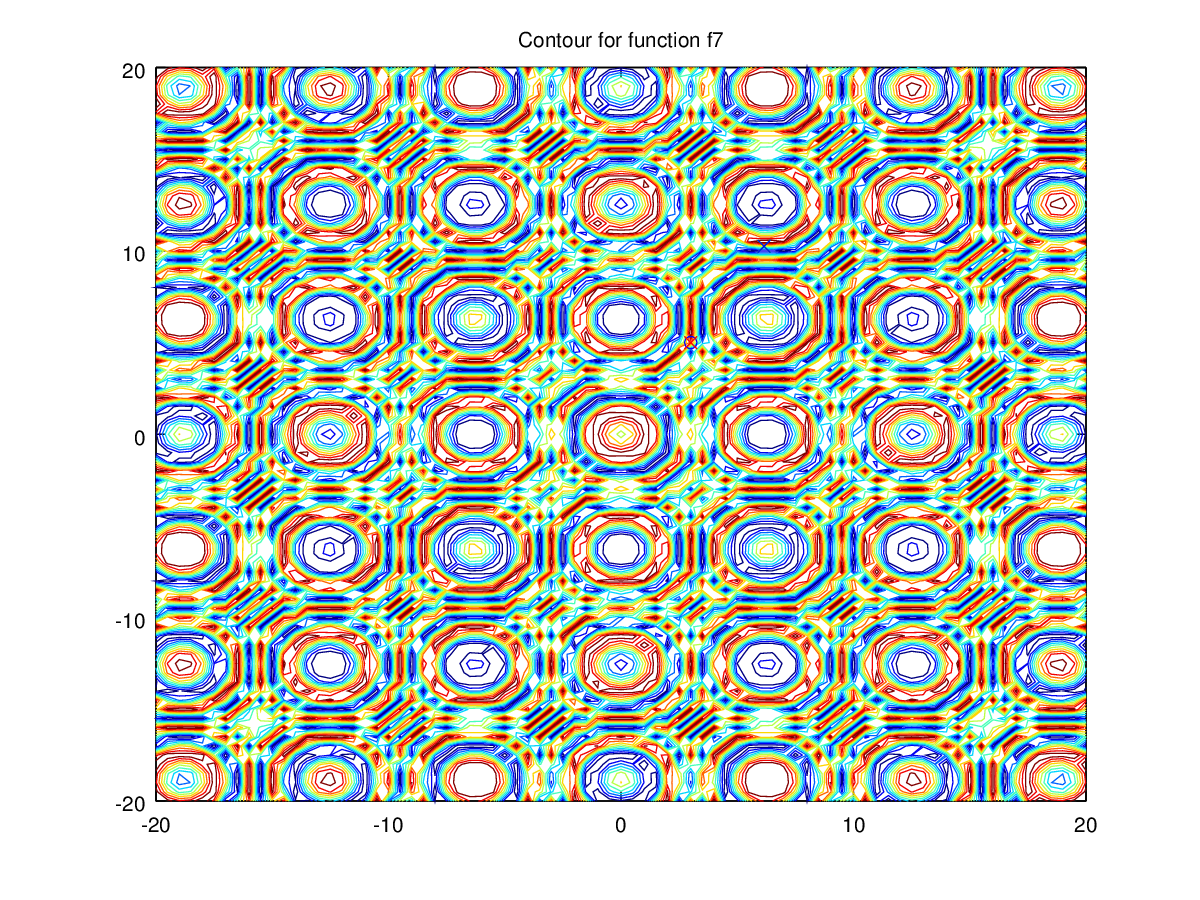
\includegraphics[width=250px]{../matlab/images/f7_contour}
  \caption{Curvas de nível para a função \autoref{eq:f7}}
  \label{fig:f7}
\end{figure}

A \autoref{tab:f7} mostra os resultados encontrados para os três algoritmos testados bem como o número de iterações gasto por cada um deles.

\begin{table}[H]
\centering
\begin{tabular}{*3c}
\toprule
Método			&	x*		&	Iterações\\
\midrule
Newton modificado	&	(2.9976, 4.9960)	&	100\\
Newton corrigido	&	(6.1513, 10.2520)	&	3\\
Quasi-newton		&	(6.1513, 10.2520)	&	3\\
\bottomrule
\end{tabular}
\caption{\small{Resultados para a função \autoref{eq:f7} }}
\label{tab:f7}
\end{table}

É possível ver que a função não é bem comportada, o que faz o método de Newton modificado gastar o número máximo de iterações e não se afasta muito
do ponto inicial. O método de Newton corrigido e o Quasi-Newton convergem para um mínimo local.

\section{Função 8}
A regra que define a função é:
\begin{equation}
\label{eq:f8}
f(x, y) = y^2(1-\cos(x)) + 1 -\cos(y) + e^{x^2}
\end{equation}

Podemos ver na \autoref{fig:f8} as curvas de nível para \autoref{eq:f8}. O símbolo \textit{\textopenbullet} marca o ponto de início,
e o símbolo \textit{\texttimes} marca o ótimo encontrado pelos três algoritmos.

\begin{figure}[H]
  \centering
  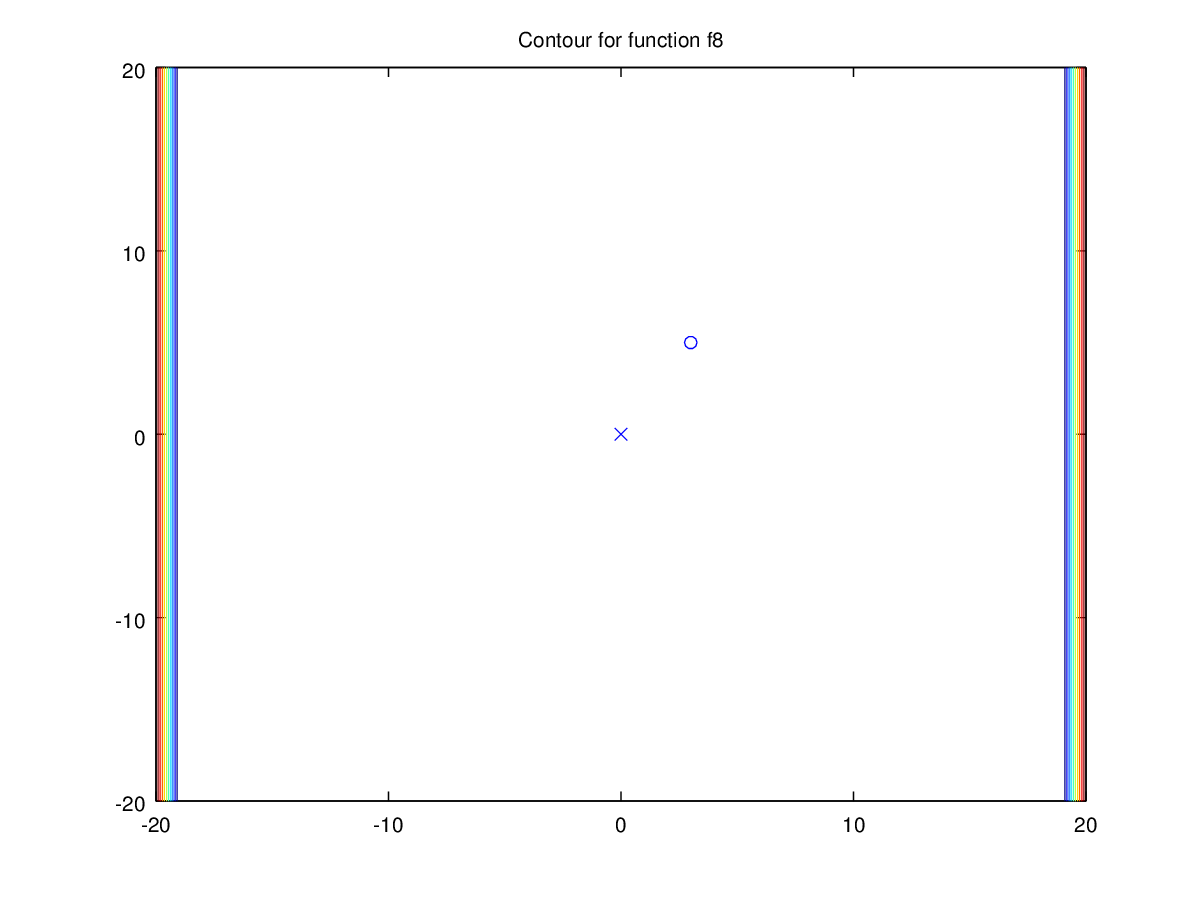
\includegraphics[width=250px]{../matlab/images/f8_contour}
  \caption{Curvas de nível para a função \autoref{eq:f8}}
  \label{fig:f8}
\end{figure}

A \autoref{tab:f8} mostra os resultados encontrados para os três algoritmos testados bem como o número de iterações gasto por cada um deles.

\begin{table}[H]
\centering
\begin{tabular}{*3c}
\toprule
Método			&	x*		&	Iterações\\
\midrule
Newton modificado	&	(-0.0000, 0.0000)	&	100\\
Newton corrigido	&	(-48597.8506, 5.9586)	&	1\\
Quasi-newton		&	(-48597.8506, 5.9586)	&	1\\
\bottomrule
\end{tabular}
\caption{\small{Resultados para a função \autoref{eq:f8} }}
\label{tab:f8}
\end{table}

Podemos ver que o método de newton conseguiu convergir para o mínimo, entretanto os métodos com correção de posto e estimativa da hessiana
tiveram problemas em caminhar no espaço. Provavelmente isso aconteceu pelo uso de \textit{pinv()} como já foi mencionado.

\section{Função 9}
A regra que define a função é:
\begin{equation}
\label{eq:f9}
f(x, y) = x^2 + y^2 - 10\cos(2\pi x) -10\cos(2\pi y)
\end{equation}

Podemos ver na \autoref{fig:f9} as curvas de nível para \autoref{eq:f9}. O símbolo \textit{\textopenbullet} marca o ponto de início,
e o símbolo \textit{\texttimes} marca o ótimo encontrado pelos três algoritmos.

\begin{figure}[H]
  \centering
  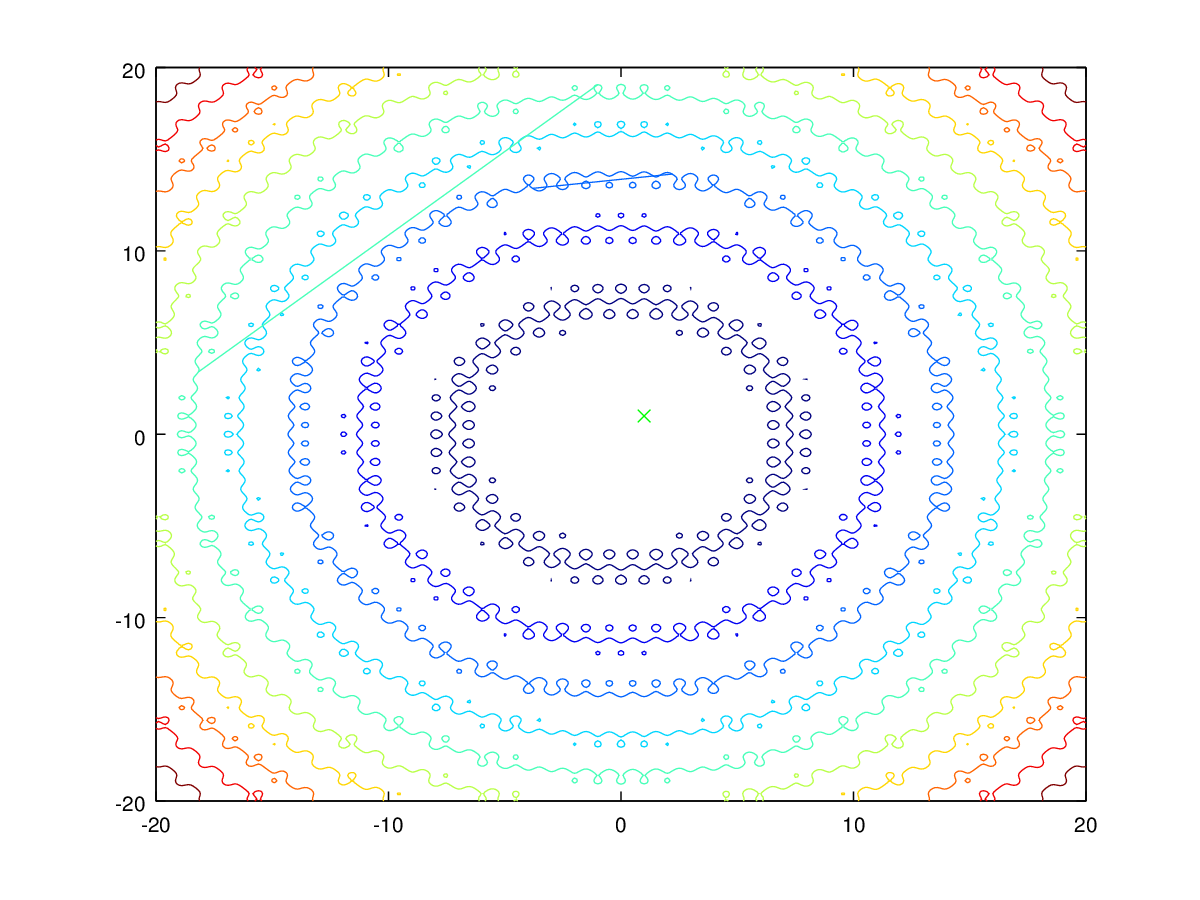
\includegraphics[width=250px]{../matlab/images/f9_contour}
  \caption{Curvas de nível para a função \autoref{eq:f9}}
  \label{fig:f9}
\end{figure}

A \autoref{tab:f9} mostra os resultados encontrados para os três algoritmos testados bem como o número de iterações gasto por cada um deles.

\begin{table}[H]
\centering
\begin{tabular}{*3c}
\toprule
Método			&	x*		&	Iterações\\
\midrule
Newton modificado	&	(2.9849, 4.9747)	&	3\\
Newton corrigido	&	(-0.0000, 0.0000)	&	4\\
Quasi-newton		&	(-0.0000, 0.0000)	&	4\\
\bottomrule
\end{tabular}
\caption{\small{Resultados para a função \autoref{eq:f9} }}
\label{tab:f9}
\end{table}

Nesta função o método de newton não conseguiu escapar do ponto de início enquanto os outros métodos alcançaram um minimo melhor.

\section{Função 10}
A regra que define a função é:
\begin{equation}
\label{eq:f10}
f(x, y) = 100(x^2 -y)^2 + (1 - x)^2
\end{equation}

Podemos ver na \autoref{fig:f10} as curvas de nível para \autoref{eq:f10}. O símbolo \textit{\textopenbullet} marca o ponto de início,
e o símbolo \textit{\texttimes} marca o ótimo encontrado pelos três algoritmos.

\begin{figure}[H]
  \centering
  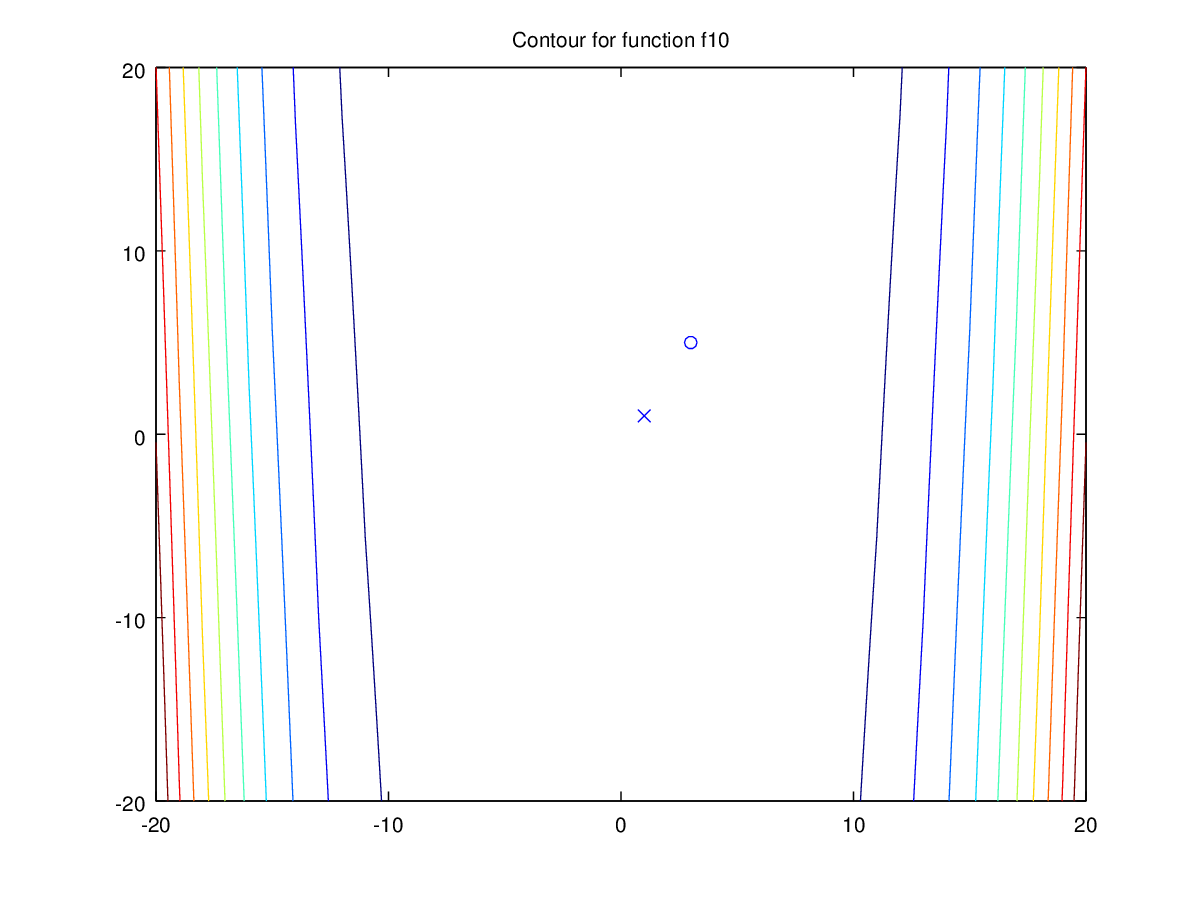
\includegraphics[width=250px]{../matlab/images/f10_contour}
  \caption{Curvas de nível para a função \autoref{eq:f10}}
  \label{fig:f10}
\end{figure}

A \autoref{tab:f10} mostra os resultados encontrados para os três algoritmos testados bem como o número de iterações gasto por cada um deles.

\begin{table}[H]
\centering
\begin{tabular}{*3c}
\toprule
Método			&	x*		&	Iterações\\
\midrule
Newton modificado	&	(0.9998, 0.9997)	&	100\\
Newton corrigido	&	(0.9997, 0.9994)	&	52\\
Quasi-newton		&	(0.9998, 0.9995)	&	100\\
\bottomrule
\end{tabular}
\caption{\small{Resultados para a função \autoref{eq:f10} }}
\label{tab:f10}
\end{table}

É possível ver que todos os métodos chegaram muito perto do ótimo mas dois deles levaram um número máximo de iterações e 
o Newton com correção do posto levou quase metade das iterações máximas, i.e., todos tiveram muita dificuldade pra alcançar o mínimo.	


\section{Função 11}
A regra que define a função é:
\begin{equation}
\label{eq:f11}
f(x, y) = 9x^2 + 4y^2 - 10\cos(6\pi x) - 10\cos(4\pi y)
\end{equation}

Podemos ver na \autoref{fig:f11} as curvas de nível para \autoref{eq:f11}. O símbolo \textit{\textopenbullet} marca o ponto de início,
e o símbolo \textit{\texttimes} marca o ótimo encontrado pelos três algoritmos.

\begin{figure}[H]
  \centering
  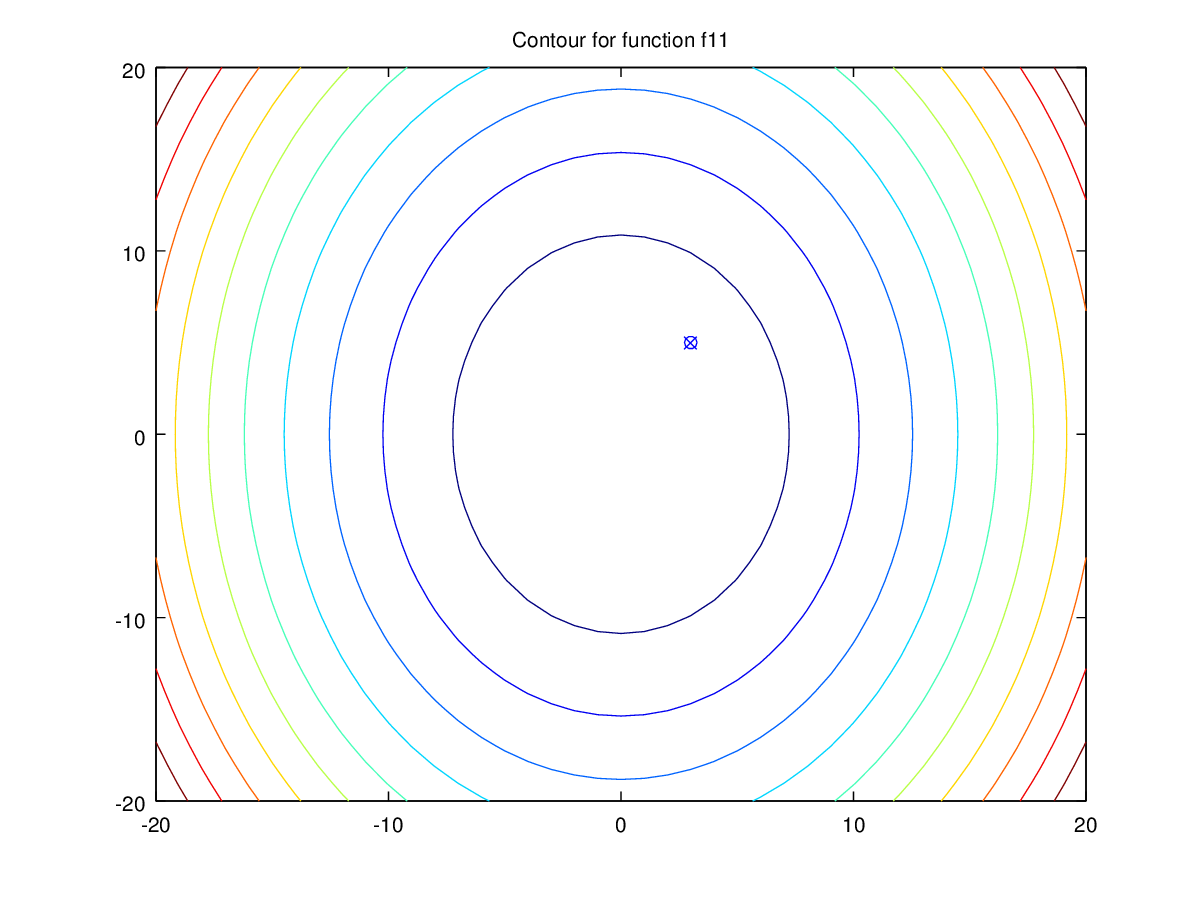
\includegraphics[width=250px]{../matlab/images/f11_contour}
  \caption{Curvas de nível para a função \autoref{eq:f11}}
  \label{fig:f11}
\end{figure}

A \autoref{tab:f11} mostra os resultados encontrados para os três algoritmos testados bem como o número de iterações gasto por cada um deles.

\begin{table}[H]
\centering
\begin{tabular}{*3c}
\toprule
Método			&	x*		&	Iterações\\
\midrule
Newton modificado	&	(2.9847, 4.9744)	&	100\\
Newton corrigido	&	(-1.6582, -0.9950)	&	9\\
Quasi-newton		&	(-0.6633, 0.0000)	&	100\\
\bottomrule
\end{tabular}
\caption{\small{Resultados para a função \autoref{eq:f11} }}
\label{tab:f11}
\end{table}

Nesta função ambos os métodos de Newton e Newton corrigido ficam presos em mínimos locais. Somente o método de Quasi-Newton se aproxima da solução
com um parando pelo número máximo de execuções.

\section{Função 12}
A regra que define a função é:
\begin{equation}
\label{eq:f12}
f(x, y) = x^2 + y^2 - 0.3\cos(3\pi x) - 0.4\cos(4\pi y) + 0.7
\end{equation}

Podemos ver na \autoref{fig:f12} as curvas de nível para \autoref{eq:f12}. O símbolo \textit{\textopenbullet} marca o ponto de início,
e o símbolo \textit{\texttimes} marca o ótimo encontrado pelos três algoritmos.

\begin{figure}[H]
  \centering
  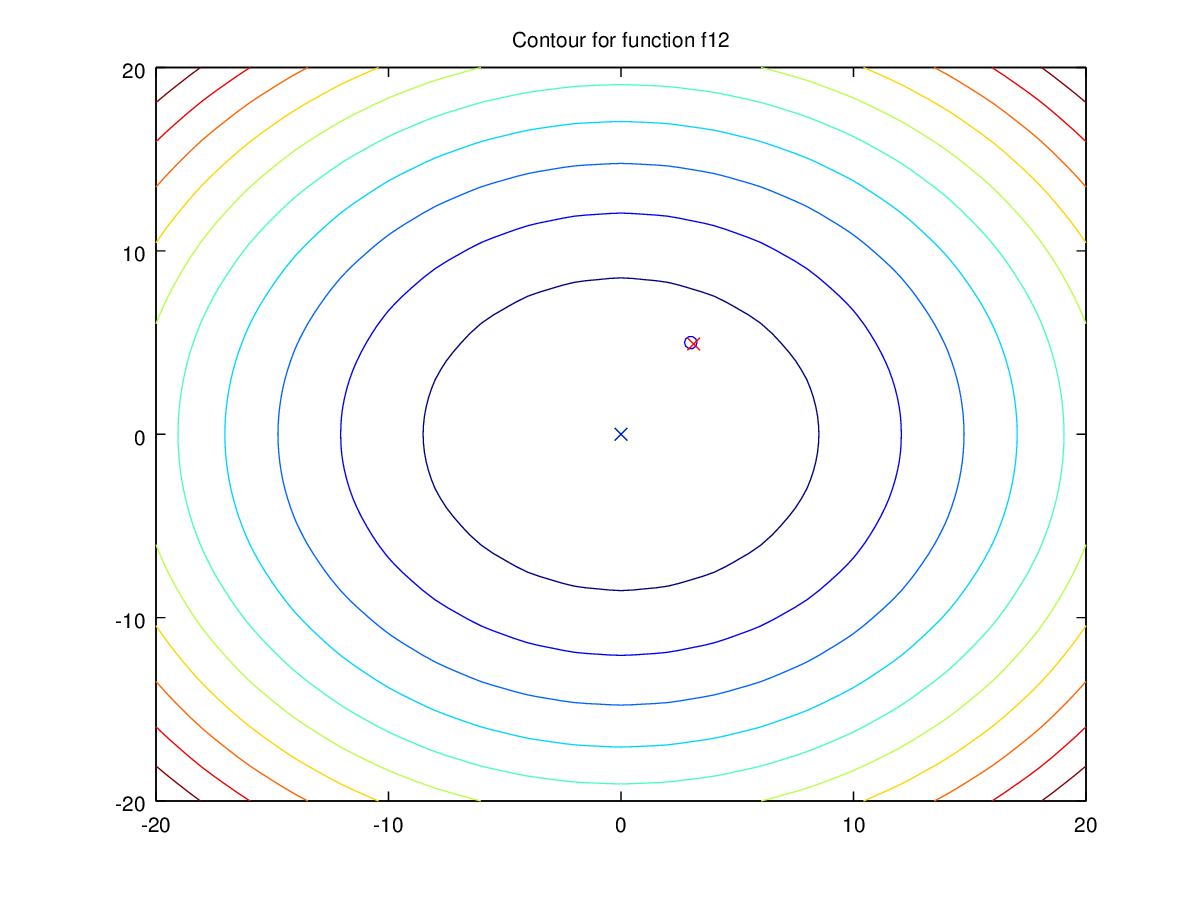
\includegraphics[width=250px]{../matlab/images/f12_contour}
  \caption{Curvas de nível para a função \autoref{eq:f12}}
  \label{fig:f12}
\end{figure}

A \autoref{tab:f12} mostra os resultados encontrados para os três algoritmos testados bem como o número de iterações gasto por cada um deles.

\begin{table}[H]
\centering
\begin{tabular}{*3c}
\toprule
Método			&	x*		&	Iterações\\
\midrule
Newton modificado	&	 (3.1247, 4.9247)	&	100\\
Newton corrigido	&	(0.0000, -0.0000)	&	3\\
Quasi-newton		&	(0.0000, -0.0000)	&	3\\
\bottomrule
\end{tabular}
\caption{\small{Resultados para a função \autoref{eq:f12} }}
\label{tab:f12}
\end{table}

Nesta função o método de newton ficou preso em um mínimo local e parou pelo número máximo de iterações. Os dois últimos métodos encontraram 
o mínimo global.

\end{document}
